\section{Results}
\label{sec:results}

\subsection{What the Symbolic Features Measure}
\label{sec:featresults}

Table~\ref{tab:features} reports group differences for all 13 features on the training split. Every
feature is significant after Holm correction, which at $n=14{,}382$ is uninformative on its own; the effect
sizes are what matter. Lexical-diversity features separate the classes most strongly (type--token ratio
$d=+0.85$, hapax ratio $d=+0.84$: hoax texts are lexically sparser \emph{relative to their length}),
followed by institutional attribution ($d=-0.62$) and the attribution/rumour ratio ($d=-0.54$): valid news
names its sources roughly five times as often as hoax text does. The morphological features behave as
predicted in direction but weakly: valid news uses more active-voice prefixes ($d=-0.31$) and more
\emph{ke-an} nominalisations ($d=-0.26$), consistent with an edited, institutional register, while passive
voice barely differs ($d=-0.06$).

The one hypothesis that clearly fails is the rumour-evidential lexicon: \emph{konon}, \emph{katanya},
\emph{dikabarkan} and their 14 companions occur at essentially identical rates in both classes
($0.078$ vs.\ $0.082$ per 100 words, $d=-0.009$) despite $p<10^{-66}$. Explicit rumour marking is not how
Indonesian hoaxes signal themselves in this corpus; the asymmetry lies in the \emph{absence} of
institutional attribution, not in the presence of rumour framing. Sensational markers do separate the
classes ($d=+0.21$) but are rare in absolute terms.

\begin{table}[t]
\centering\small
\caption{Group differences on the \iph{} training split ($n_{\text{hoax}}=7{,}612$, $n_{\text{valid}}=6{,}770$).
Means are per 100 words for rate features. $d$ is Cohen's $d$ (hoax $-$ valid) with a 95\% confidence
interval; $p$ is the Holm-corrected Mann--Whitney $U$ $p$-value. Rows are ordered by $|d|$.}
\label{tab:features}
\begin{tabular}{lrrrcr}
\toprule
Feature & Hoax & Valid & $d$ & 95\% CI & $p_{\text{Holm}}$ \\
\midrule
Type-token ratio & 0.790 & 0.668 & +0.845 & [+0.810, +0.879] & $<$0.001 \\
Hapax legomena ratio & 0.672 & 0.503 & +0.842 & [+0.808, +0.876] & $<$0.001 \\
Institutional attribution & 0.074 & 0.343 & -0.619 & [-0.652, -0.585] & $<$0.001 \\
Attribution/rumour ratio & 7.326 & 30.291 & -0.540 & [-0.573, -0.506] & $<$0.001 \\
Word count & 138.127 & 220.594 & -0.462 & [-0.495, -0.429] & $<$0.001 \\
Character count & 993.461 & 1577.578 & -0.452 & [-0.485, -0.419] & $<$0.001 \\
Active prefix (meN-/ber-) & 3.184 & 4.071 & -0.312 & [-0.345, -0.279] & $<$0.001 \\
Nominal circumfix ke-an & 0.867 & 1.275 & -0.256 & [-0.289, -0.223] & $<$0.001 \\
Sensational markers & 0.228 & 0.027 & +0.207 & [+0.174, +0.240] & $<$0.001 \\
Avg. word length & 5.875 & 5.933 & -0.078 & [-0.111, -0.045] & $<$0.001 \\
Passive prefix (di-/ter-) & 2.737 & 2.879 & -0.056 & [-0.088, -0.023] & $<$0.001 \\
Discourse particles & 0.407 & 0.317 & +0.054 & [+0.021, +0.087] & $<$0.001 \\
Rumour evidentials & 0.078 & 0.082 & -0.009 & [-0.041, +0.024] & $<$0.001 \\
\bottomrule
\end{tabular}%

\end{table}

\begin{figure}[t]
\centering
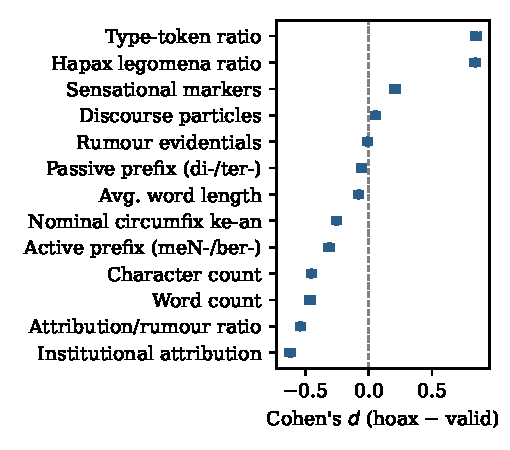
\includegraphics[width=0.62\linewidth]{figures/effect_sizes.pdf}
\caption{Effect sizes with 95\% confidence intervals. Positive values indicate higher values in hoax text.
Rumour evidentials, the feature group we expected to be most diagnostic, are indistinguishable between
classes.}
\label{fig:effects}
\end{figure}

\subsection{In-Domain Results}
\label{sec:indomain}

Tables~\ref{tab:main-original} and \ref{tab:main-normalized} give the main comparison. On the
de-duplicated \iph{} test split every model that sees tokens lands in a narrow band around
macro-F1 $0.974$--$0.978$: \menet{} reaches $0.9761{\pm}0.0054$, the text-only CNN $0.9738{\pm}0.0031$,
naive concatenation $0.9778{\pm}0.0015$ and TF-IDF with logistic regression $0.9749$. Fine-tuned
IndoBERT is the only model clearly above that band. None of the paired comparisons between \menet{} and
its ablations survives Holm correction in any condition (Table~\ref{tab:sig}): the largest absolute mean
difference is $1.4$ F1 points (\menet{} vs.\ \emph{w/o length features}, cross-dataset, normalised text,
$p_{\text{Holm}}=0.32$) and the in-domain differences are all below $0.3$ points. \textbf{On this
benchmark the gate, the symbolic stream and the individual feature groups make no measurable difference to
accuracy.} We report this as the primary empirical finding rather than searching for a condition in which
the proposed model wins.

Two secondary observations do hold consistently. First, the fused models are better calibrated than the
linear text baseline: ECE $0.012$ for the \menet{} family versus $0.053$ for TF-IDF$+$LR, a factor of four,
at equal accuracy. Second, the symbolic stream alone is far from trivial: 13 numbers with no lexical
content give macro-F1 $0.789{\pm}0.008$ (MLP) and $0.718$ (logistic regression), i.e.\ roughly
four-fifths of full performance from a 3{,}137-parameter model.

\subsection{Evidence of Shortcuts}
\label{sec:shortcuts}

The narrow band above is easier to interpret next to two controls. A logistic regression on \emph{two
features}, word count and character count, reaches macro-F1 $0.638$ in-domain, and format normalisation
changes almost nothing anywhere: the CNN moves from $0.9738$ to $0.9738$ and \menet{} from $0.9761$ to
$0.9763$, so casing and punctuation are not the carrier of the signal, but length and topic-specific
vocabulary are available in both views. In other words, a substantial part of what any model learns here
is a property of how the corpus was assembled (short social-media hoax posts versus long wire-service
articles), not of deceptive language as such \citep{gururangan2018annotation,geirhos2020shortcut}.

Cross-dataset transfer confirms this. On Rahutomo-600, where both classes are full-length articles
labelled by referees rather than scraped from different pipelines, every system collapses towards chance:
\menet{} $0.521{\pm}0.015$, the CNN $0.520{\pm}0.012$, naive concatenation $0.532{\pm}0.011$,
TF-IDF$+$LR $0.548$, and IndoBERT, the strongest in-domain model by a wide margin, $0.557$. The ranking
in-domain therefore carries essentially no information about transfer, and a 124M-parameter transformer
buys nothing out of domain despite a $+1.7$-point in-domain advantage. Calibration degrades in parallel:
ECE rises from $0.012$ to $0.288$ for \menet{} and from $0.007$ to $0.401$ for IndoBERT, so the models are
not merely wrong out of domain, they are confidently wrong. The symbolic-only models are the exception
worth noting: at chance-level accuracy they remain comparatively calibrated (ECE $0.15$--$0.19$).

\begin{figure}[t]
\centering
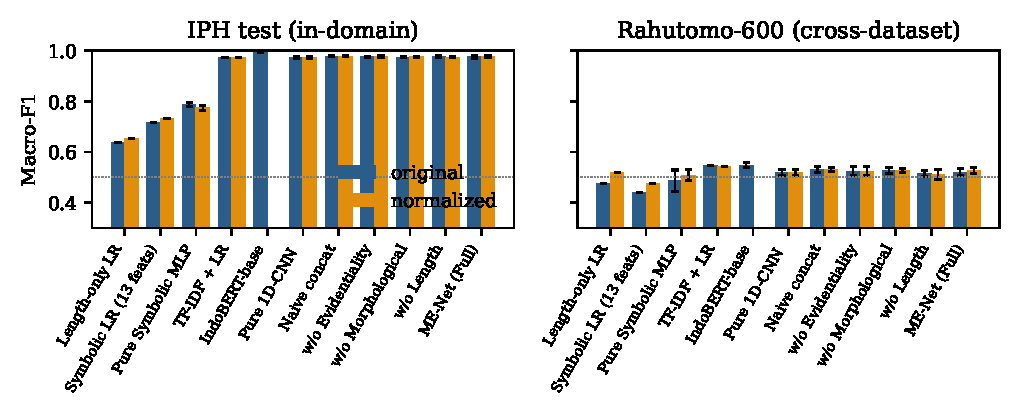
\includegraphics[width=\linewidth]{figures/indomain_vs_crossdataset.pdf}
\caption{Macro-F1 in-domain (left) and cross-dataset (right) for both input settings; bars are means over
seeds with standard-deviation whiskers. The dotted line marks chance-level macro-F1. In-domain separation
between token-based models is within noise, and no model transfers.}
\label{fig:indomain-vs-ood}
\end{figure}

\subsection{What the Gate Learns}
\label{sec:gateresults}

Because $\bar g$ of Eq.~\eqref{eq:gbar} is part of the forward pass, we can ask what the trained model
relies on without post-hoc attribution. Averaged over 10 seeds, the mean gate is
$\bar g=0.326{\pm}0.020$ for documents labelled hoax and $0.389{\pm}0.045$ for valid ones on the
in-domain test set: both classes sit below $0.5$, i.e.\ the fused representation is drawn more from the
symbolic stream than from the contextual one, and the shift between classes is small but systematic
across seeds (Figure~\ref{fig:gate}). On Rahutomo-600 the class difference vanishes
($0.361{\pm}0.034$ vs.\ $0.359{\pm}0.033$), matching the accuracy collapse: out of domain the gate no
longer discriminates, which is exactly the diagnostic signature one would want from an interpretable
component. The gate thus does something measurable and inspectable, even though it does not translate
into an accuracy gain here.

\begin{figure}[t]
\centering
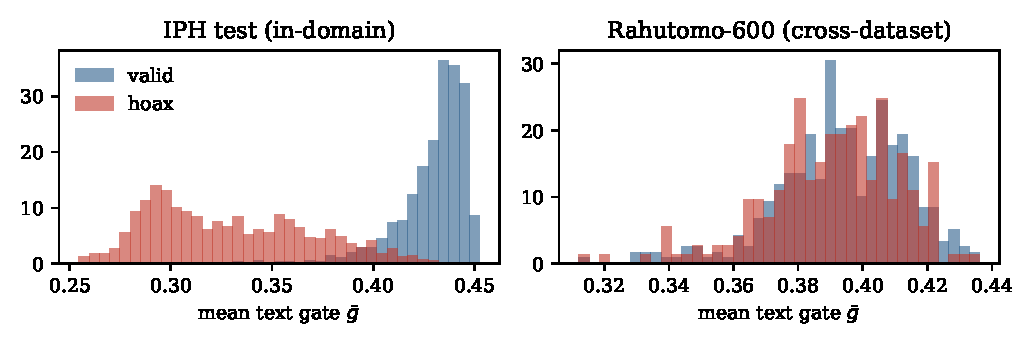
\includegraphics[width=\linewidth]{figures/gate_distribution.pdf}
\caption{Distribution of the mean gate $\bar g$ per document (first seed). In-domain (left) the two classes
separate slightly; cross-dataset (right) they coincide.}
\label{fig:gate}
\end{figure}

\subsection{Cost}
\label{sec:cost}

\menet{} has 4.03M parameters and trains in $3.6$s per run on one GPU, versus $2.2$s for the text-only CNN
and $374$s for IndoBERT (124M parameters), i.e.\ the symbolic stream and gate cost about 60\% more training
time than a bare CNN and two orders of magnitude less than fine-tuning a transformer, while the profiler
itself is a single linear pass over the text.

\begin{table}[t]
\centering\small
\caption{Main results on original text. Mean $\pm$ standard deviation over $n$ seeds (deterministic models
have $n{=}1$). Best per column in bold; ECE lower is better.}
\label{tab:main-original}
\begin{adjustbox}{max width=\linewidth}
\begin{tabular}{lccccccc}
\toprule
& & \multicolumn{3}{c}{\iph{} test (in-domain)} & \multicolumn{3}{c}{Rahutomo-600 (cross-dataset)} \\
\cmidrule(lr){3-5}\cmidrule(lr){6-8}
Model & $n$ & Macro-F1 & ROC-AUC & ECE & Macro-F1 & ROC-AUC & ECE \\
\midrule
Length-only LR & 1 & 0.638 & 0.757 & 0.099 & 0.477 & 0.447 & \textbf{0.113} \\
Symbolic LR (13 feats) & 1 & 0.718 & 0.796 & 0.053 & 0.439 & 0.488 & 0.146 \\
Pure Symbolic MLP & 10 & 0.788\,{\scriptsize$\pm$0.008} & 0.859\,{\scriptsize$\pm$0.005} & 0.066\,{\scriptsize$\pm$0.010} & 0.487\,{\scriptsize$\pm$0.042} & 0.544\,{\scriptsize$\pm$0.011} & 0.185\,{\scriptsize$\pm$0.011} \\
\midrule
TF-IDF + LR & 1 & 0.975 & 0.998 & 0.053 & 0.548 & 0.543 & 0.174 \\
IndoBERT-base (fine-tuned) & 2 & \textbf{0.992\,{\scriptsize$\pm$0.000}} & \textbf{1.000\,{\scriptsize$\pm$0.000}} & \textbf{0.008\,{\scriptsize$\pm$0.000}} & \textbf{0.549\,{\scriptsize$\pm$0.012}} & \textbf{0.595\,{\scriptsize$\pm$0.001}} & 0.404\,{\scriptsize$\pm$0.005} \\
\midrule
Pure 1D-CNN (w/o Symbolic) & 10 & 0.974\,{\scriptsize$\pm$0.003} & 0.997\,{\scriptsize$\pm$0.000} & 0.013\,{\scriptsize$\pm$0.002} & 0.520\,{\scriptsize$\pm$0.012} & 0.546\,{\scriptsize$\pm$0.009} & 0.320\,{\scriptsize$\pm$0.021} \\
Naive Concatenation (w/o Gate) & 10 & 0.978\,{\scriptsize$\pm$0.002} & 0.998\,{\scriptsize$\pm$0.000} & 0.011\,{\scriptsize$\pm$0.002} & 0.532\,{\scriptsize$\pm$0.011} & 0.558\,{\scriptsize$\pm$0.009} & 0.288\,{\scriptsize$\pm$0.013} \\
ME-Net w/o Evidentiality Priors & 10 & 0.975\,{\scriptsize$\pm$0.002} & 0.997\,{\scriptsize$\pm$0.000} & 0.013\,{\scriptsize$\pm$0.003} & 0.525\,{\scriptsize$\pm$0.018} & 0.547\,{\scriptsize$\pm$0.011} & 0.303\,{\scriptsize$\pm$0.024} \\
ME-Net w/o Morphological Priors & 10 & 0.975\,{\scriptsize$\pm$0.003} & 0.997\,{\scriptsize$\pm$0.000} & 0.014\,{\scriptsize$\pm$0.003} & 0.527\,{\scriptsize$\pm$0.012} & 0.551\,{\scriptsize$\pm$0.008} & 0.294\,{\scriptsize$\pm$0.024} \\
ME-Net w/o Length Features & 10 & 0.977\,{\scriptsize$\pm$0.004} & 0.997\,{\scriptsize$\pm$0.000} & 0.014\,{\scriptsize$\pm$0.002} & 0.516\,{\scriptsize$\pm$0.011} & 0.544\,{\scriptsize$\pm$0.008} & 0.309\,{\scriptsize$\pm$0.012} \\
\midrule
ME-Net (Full) & 10 & 0.976\,{\scriptsize$\pm$0.005} & 0.997\,{\scriptsize$\pm$0.000} & 0.012\,{\scriptsize$\pm$0.003} & 0.521\,{\scriptsize$\pm$0.015} & 0.557\,{\scriptsize$\pm$0.007} & 0.288\,{\scriptsize$\pm$0.024} \\
\bottomrule
\end{tabular}%

\end{adjustbox}
\end{table}

\begin{table}[t]
\centering\small
\caption{Main results on format-normalised text (lower-cased, punctuation removed).}
\label{tab:main-normalized}
\begin{adjustbox}{max width=\linewidth}
\begin{tabular}{lccccccc}
\toprule
& & \multicolumn{3}{c}{\iph{} test (in-domain)} & \multicolumn{3}{c}{Rahutomo-600 (cross-dataset)} \\
\cmidrule(lr){3-5}\cmidrule(lr){6-8}
Model & $n$ & Macro-F1 & ROC-AUC & ECE & Macro-F1 & ROC-AUC & ECE \\
\midrule
Length-only LR & 1 & 0.654 & 0.783 & 0.117 & 0.521 & 0.484 & \textbf{0.104} \\
Symbolic LR (13 feats) & 1 & 0.733 & 0.799 & 0.057 & 0.475 & 0.529 & 0.115 \\
Pure Symbolic MLP & 10 & 0.775\,{\scriptsize$\pm$0.011} & 0.846\,{\scriptsize$\pm$0.005} & 0.074\,{\scriptsize$\pm$0.014} & 0.509\,{\scriptsize$\pm$0.022} & 0.554\,{\scriptsize$\pm$0.004} & 0.148\,{\scriptsize$\pm$0.011} \\
\midrule
TF-IDF + LR & 1 & 0.975 & \textbf{0.998} & 0.053 & \textbf{0.544} & 0.544 & 0.164 \\
\midrule
Pure 1D-CNN (w/o Symbolic) & 10 & 0.974\,{\scriptsize$\pm$0.003} & 0.997\,{\scriptsize$\pm$0.000} & 0.013\,{\scriptsize$\pm$0.002} & 0.520\,{\scriptsize$\pm$0.012} & 0.546\,{\scriptsize$\pm$0.009} & 0.320\,{\scriptsize$\pm$0.021} \\
Naive Concatenation (w/o Gate) & 10 & \textbf{0.978\,{\scriptsize$\pm$0.001}} & 0.998\,{\scriptsize$\pm$0.000} & \textbf{0.012\,{\scriptsize$\pm$0.002}} & 0.530\,{\scriptsize$\pm$0.008} & 0.557\,{\scriptsize$\pm$0.008} & 0.298\,{\scriptsize$\pm$0.013} \\
ME-Net w/o Evidentiality Priors & 10 & 0.976\,{\scriptsize$\pm$0.003} & 0.997\,{\scriptsize$\pm$0.000} & 0.014\,{\scriptsize$\pm$0.002} & 0.525\,{\scriptsize$\pm$0.018} & 0.547\,{\scriptsize$\pm$0.010} & 0.311\,{\scriptsize$\pm$0.021} \\
ME-Net w/o Morphological Priors & 10 & 0.975\,{\scriptsize$\pm$0.003} & 0.997\,{\scriptsize$\pm$0.000} & 0.012\,{\scriptsize$\pm$0.003} & 0.527\,{\scriptsize$\pm$0.007} & 0.556\,{\scriptsize$\pm$0.007} & 0.299\,{\scriptsize$\pm$0.027} \\
ME-Net w/o Length Features & 10 & 0.975\,{\scriptsize$\pm$0.004} & 0.997\,{\scriptsize$\pm$0.000} & 0.012\,{\scriptsize$\pm$0.003} & 0.512\,{\scriptsize$\pm$0.019} & 0.551\,{\scriptsize$\pm$0.010} & 0.322\,{\scriptsize$\pm$0.030} \\
\midrule
ME-Net (Full) & 10 & 0.976\,{\scriptsize$\pm$0.004} & 0.997\,{\scriptsize$\pm$0.000} & 0.012\,{\scriptsize$\pm$0.002} & 0.527\,{\scriptsize$\pm$0.011} & \textbf{0.561\,{\scriptsize$\pm$0.006}} & 0.296\,{\scriptsize$\pm$0.028} \\
\bottomrule
\end{tabular}%

\end{adjustbox}
\end{table}

\begin{table}[t]
\centering\small
\caption{Paired differences in macro-F1 (percentage points) between \menet{} and each ablation over the
same 10 seeds, with the number of seeds on which \menet{} is better. Positive means \menet{} is better.
$^{*}$ marks $p_{\text{Holm}}<0.05$ (two-sided Wilcoxon signed-rank, corrected over the five comparisons
per condition); no comparison reaches it.}
\label{tab:sig}
\begin{adjustbox}{max width=\linewidth}
\begin{tabular}{lcccc}
\toprule
& \multicolumn{2}{c}{Original text} & \multicolumn{2}{c}{Normalised text} \\
\cmidrule(lr){2-3}\cmidrule(lr){4-5}
Comparison (\menet{} $-$ variant) & in-domain & cross-dataset & in-domain & cross-dataset \\
\midrule
Pure 1D-CNN (w/o Symbolic) & +0.23 (6/10) & +0.16 (5/10) & +0.25 (6/10) & +0.71 (6/10) \\
Naive Concatenation (w/o Gate) & -0.18 (4/10) & -1.11 (2/10) & -0.14 (3/10) & -0.32 (4/10) \\
ME-Net w/o Evidentiality Priors & +0.07 (5/10) & -0.39 (3/10) & -0.01 (4/10) & +0.17 (5/10) \\
ME-Net w/o Morphological Priors & +0.13 (4/10) & -0.59 (4/10) & +0.09 (7/10) & -0.08 (5/10) \\
ME-Net w/o Length Features & -0.09 (5/10) & +0.51 (5/10) & +0.12 (5/10) & +1.41 (7/10) \\
\bottomrule
\end{tabular}%

\end{adjustbox}
\end{table}
